% Options for packages loaded elsewhere
\PassOptionsToPackage{unicode}{hyperref}
\PassOptionsToPackage{hyphens}{url}
\PassOptionsToPackage{dvipsnames,svgnames,x11names}{xcolor}
%
\documentclass[
  letterpaper,
  DIV=11,
  numbers=noendperiod,
  oneside]{scrartcl}

\usepackage{amsmath,amssymb}
\usepackage{iftex}
\ifPDFTeX
  \usepackage[T1]{fontenc}
  \usepackage[utf8]{inputenc}
  \usepackage{textcomp} % provide euro and other symbols
\else % if luatex or xetex
  \usepackage{unicode-math}
  \defaultfontfeatures{Scale=MatchLowercase}
  \defaultfontfeatures[\rmfamily]{Ligatures=TeX,Scale=1}
\fi
\usepackage{lmodern}
\ifPDFTeX\else  
    % xetex/luatex font selection
\fi
% Use upquote if available, for straight quotes in verbatim environments
\IfFileExists{upquote.sty}{\usepackage{upquote}}{}
\IfFileExists{microtype.sty}{% use microtype if available
  \usepackage[]{microtype}
  \UseMicrotypeSet[protrusion]{basicmath} % disable protrusion for tt fonts
}{}
\makeatletter
\@ifundefined{KOMAClassName}{% if non-KOMA class
  \IfFileExists{parskip.sty}{%
    \usepackage{parskip}
  }{% else
    \setlength{\parindent}{0pt}
    \setlength{\parskip}{6pt plus 2pt minus 1pt}}
}{% if KOMA class
  \KOMAoptions{parskip=half}}
\makeatother
\usepackage{xcolor}
\usepackage[top=30mm,bottom=30mm,left=15mm,right=80mm,marginparwidth=60mm,marginparsep=10mm,heightrounded]{geometry}
\setlength{\emergencystretch}{3em} % prevent overfull lines
\setcounter{secnumdepth}{-\maxdimen} % remove section numbering
% Make \paragraph and \subparagraph free-standing
\makeatletter
\ifx\paragraph\undefined\else
  \let\oldparagraph\paragraph
  \renewcommand{\paragraph}{
    \@ifstar
      \xxxParagraphStar
      \xxxParagraphNoStar
  }
  \newcommand{\xxxParagraphStar}[1]{\oldparagraph*{#1}\mbox{}}
  \newcommand{\xxxParagraphNoStar}[1]{\oldparagraph{#1}\mbox{}}
\fi
\ifx\subparagraph\undefined\else
  \let\oldsubparagraph\subparagraph
  \renewcommand{\subparagraph}{
    \@ifstar
      \xxxSubParagraphStar
      \xxxSubParagraphNoStar
  }
  \newcommand{\xxxSubParagraphStar}[1]{\oldsubparagraph*{#1}\mbox{}}
  \newcommand{\xxxSubParagraphNoStar}[1]{\oldsubparagraph{#1}\mbox{}}
\fi
\makeatother


\providecommand{\tightlist}{%
  \setlength{\itemsep}{0pt}\setlength{\parskip}{0pt}}\usepackage{longtable,booktabs,array}
\usepackage{calc} % for calculating minipage widths
% Correct order of tables after \paragraph or \subparagraph
\usepackage{etoolbox}
\makeatletter
\patchcmd\longtable{\par}{\if@noskipsec\mbox{}\fi\par}{}{}
\makeatother
% Allow footnotes in longtable head/foot
\IfFileExists{footnotehyper.sty}{\usepackage{footnotehyper}}{\usepackage{footnote}}
\makesavenoteenv{longtable}
\usepackage{graphicx}
\makeatletter
\def\maxwidth{\ifdim\Gin@nat@width>\linewidth\linewidth\else\Gin@nat@width\fi}
\def\maxheight{\ifdim\Gin@nat@height>\textheight\textheight\else\Gin@nat@height\fi}
\makeatother
% Scale images if necessary, so that they will not overflow the page
% margins by default, and it is still possible to overwrite the defaults
% using explicit options in \includegraphics[width, height, ...]{}
\setkeys{Gin}{width=\maxwidth,height=\maxheight,keepaspectratio}
% Set default figure placement to htbp
\makeatletter
\def\fps@figure{htbp}
\makeatother

\usepackage{lastpage}
\usepackage{fancyhdr}
\usepackage{titling}
\pagestyle{fancy}
\fancyhead[L]{CMPE2150 Notes 05}
\fancyhead[R]{Semiconductor AC Control}
\fancyfoot[C]{\thepage/\pageref*{LastPage}}
\setlength{\droptitle}{-2cm}
\KOMAoption{captions}{tablesignature}
\makeatletter
\@ifpackageloaded{caption}{}{\usepackage{caption}}
\AtBeginDocument{%
\ifdefined\contentsname
  \renewcommand*\contentsname{Table of contents}
\else
  \newcommand\contentsname{Table of contents}
\fi
\ifdefined\listfigurename
  \renewcommand*\listfigurename{List of Figures}
\else
  \newcommand\listfigurename{List of Figures}
\fi
\ifdefined\listtablename
  \renewcommand*\listtablename{List of Tables}
\else
  \newcommand\listtablename{List of Tables}
\fi
\ifdefined\figurename
  \renewcommand*\figurename{Figure}
\else
  \newcommand\figurename{Figure}
\fi
\ifdefined\tablename
  \renewcommand*\tablename{Table}
\else
  \newcommand\tablename{Table}
\fi
}
\@ifpackageloaded{float}{}{\usepackage{float}}
\floatstyle{ruled}
\@ifundefined{c@chapter}{\newfloat{codelisting}{h}{lop}}{\newfloat{codelisting}{h}{lop}[chapter]}
\floatname{codelisting}{Listing}
\newcommand*\listoflistings{\listof{codelisting}{List of Listings}}
\makeatother
\makeatletter
\makeatother
\makeatletter
\@ifpackageloaded{caption}{}{\usepackage{caption}}
\@ifpackageloaded{subcaption}{}{\usepackage{subcaption}}
\makeatother
\makeatletter
\@ifpackageloaded{sidenotes}{}{\usepackage{sidenotes}}
\@ifpackageloaded{marginnote}{}{\usepackage{marginnote}}
\makeatother

\ifLuaTeX
  \usepackage{selnolig}  % disable illegal ligatures
\fi
\usepackage{bookmark}

\IfFileExists{xurl.sty}{\usepackage{xurl}}{} % add URL line breaks if available
\urlstyle{same} % disable monospaced font for URLs
\hypersetup{
  pdftitle={CMPE2150 Notes 05},
  pdfauthor={Taylor, Moore, and Armstrong},
  colorlinks=true,
  linkcolor={blue},
  filecolor={Maroon},
  citecolor={Blue},
  urlcolor={Blue},
  pdfcreator={LaTeX via pandoc}}


\title{CMPE2150 Notes 05}
\usepackage{etoolbox}
\makeatletter
\providecommand{\subtitle}[1]{% add subtitle to \maketitle
  \apptocmd{\@title}{\par {\large #1 \par}}{}{}
}
\makeatother
\subtitle{Semiconductor AC Control}
\author{Taylor, Moore, and Armstrong}
\date{16 Oct 2024}

\begin{document}
\maketitle

\renewcommand*\contentsname{Table of contents}
{
\hypersetup{linkcolor=}
\setcounter{tocdepth}{3}
\tableofcontents
}

\subsection{Semiconductor AC Power
Controllers}\label{semiconductor-ac-power-controllers}

Practically everything you've done in your previous work with
semiconductor devices has involved DC power. We used diodes to convert
AC power to DC power, but beyond that, we've powered BJT circuits, FET
circuits, Op Amp Circuits, Comparator circuits, and Logic circuits using
DC---either with carefully-regulated power supplies or batteries. Yes,
we've used some of these devices to manipulate AC signals, but they've
always been powered using DC.

Many devices used commercially or industrially are designed to run on AC
power. Up to this point in your study of electricity and electronics,
the only ways we've used to turn AC power on and off have been switches,
relays, and SSRs. We haven't even tried to control AC power over a range
of values (analog), as switches and relays can only be on or off
(binary).

However, you've likely encountered full-range AC power controllers as
implemented in the home: You may have a room in your house with a dimmer
for the lights instead of a switch, you may have a floor lamp with a
dimmer, and your high-efficiency furnace may speed up and slow down the
fan as it goes through its heating cycle. In industry, huge three-phase
AC motors may have speed controllers that can be manipulated by the
operator or by control circuitry.

\subsubsection{Four and Five Layer Semiconductor
Devices}\label{four-and-five-layer-semiconductor-devices}

The BJT transistors you studied earlier are three-layer devices, either
PNP or NPN. As such, they must be biased appropriately with DC power
supplies: For an NPN transistor, the Collector must be at a higher
voltage than the Emitter, and control is exercised by running a current
through the positively-biased Base to Emitter junction. For a PNP
transistor, the Collector must be at a lower voltage than the Emitter,
and control is exercised by running a current through the
negatively-biased Base to Emitter junction.

\marginnote{\begin{footnotesize}

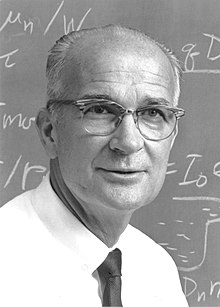
\includegraphics[width=40mm,height=\textheight]{images/William_Shockley.jpg}

William Shockley, 1910-1989 (Wikipedia)

\end{footnotesize}}

William Shockley was a researcher at Bell Labs, and, beyond his role in
inventing transistors, he had a particular interest in AC power control.
He invented a number of semiconductor devices that had more than three
layers. Some of his devices were four-layer (NPNP or PNPN) and some were
five-layer (NPNPN or PNPNP). It turned out that these devices responded
in surprising but useful ways to AC signals.

Some sources use the general term \emph{Thyristor} to include all of the
four- and five-layer devices, whereas other sources use the term for
only one of these---the Silicon Controlled Regulator(SCR). Because of
this uncertainty in terminology, we'll use specific names for all of
these devices.

All these devices (with the exception of two which have been specially
designed to have shut-off control) have this unusual characteristic in
common: once they have been activated, they remain ON until the voltage
across them drops practically to zero. Therefore, they are not
particularly useful for DC circuits -- activate the device, and you
can't turn it off! Of course, creative people have come up with ways to
use these devices in DC circuits, but they are definitely best used in
AC circuits.

In an AC circuit, the supply voltage crosses zero twice each cycle, or
120 times per second in North America. So, in an AC application, these
devices, when activated, will be turned off 120 times a second, ready to
be activated again.

Although these devices can be approximately modelled as pairs of coupled
transistors, the model sometimes doesn't adequately explain the
operation of the device, so that particular model will not be presented
in this course. If you're interested, you can look it up for yourself.
Instead, we will simply describe the behaviour of each device from an
operational point of view ---``this is what it does''---rather than from
a theoretical point of view---``this is why''.

\subsubsection{Four-layer Half-Wave AC Power
Controllers}\label{four-layer-half-wave-ac-power-controllers}

The four-layer devices can control only one polarity of the AC signal.
Typically, this is the positive half wave, with the negative half wave
producing no useful power. It is also possible to use these devices to
control the negative half wave, with the positive half wave producing no
useful power, but that is much less common.

\paragraph{Shockley Diode}\label{shockley-diode}

The basic four-layer device is called the Shockley Diode\sidenote{\footnotesize Don't
  confuse the \emph{Shockley} Diode with the \emph{Schottky} Diode,
  which is a special high-frequency/high power diode using a P-Type to
  metal junction.} , although it is not actually a diode (the names of
these devices can be a bit confusing, as you will see).

The Shockley Diode has only two pins, and is given the symbol shown in
the margin.

\marginnote{\begin{footnotesize}

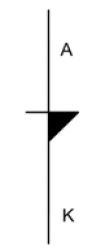
\includegraphics[width=15mm,height=\textheight]{images/ShockleySymbol.jpg}

Symbol for a Shockley Diode

\end{footnotesize}}

To begin with, the device is open, allowing no current to flow. As the
Anode to Cathode voltage increases, it remains OPEN until a relatively
large breakover voltage (\(V_{BR_f}\)) is reached and sufficient current
is injected into the Gate to turn the device on; after this, it
continues to conduct until the current is turned off or the Anode to
Cathode voltage is reduced to practically zero. The graph of the
transfer below demonstrates this.

Note the following:

\begin{itemize}
\item
  This curve is not ``reversible''.

  \begin{itemize}
  \item
    It starts at (0,0), follows an increase in VAK up to the forward
    breakover voltage \(V_{BR_f}\) and the injection of current \(I_H\).
  \item
    \(V_{AK}\) then drops to a much lower value, \(V_F\), as it has now
    been turned On.
  \item
    If biased properly, sufficient current now flows to ``hold'' it in
    the On condition---\(I_H\).
  \item
    If the voltage across the device is dropped to zero, the cycle can
    start over again at (0,0).
  \end{itemize}
\end{itemize}

\begin{figure}[H]

\sidecaption{Shockley Diode Transfer Function}

{\centering 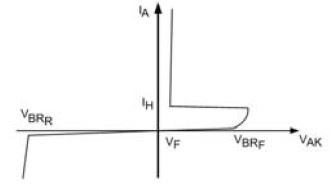
\includegraphics[width=100mm,height=\textheight]{images/ShockleyTransfer.JPG}

}

\end{figure}%

\begin{itemize}
\item
  As with other semiconductor devices you've investigated, there is also
  a reverse breakdown voltage, \(V_{BR_r}\) which should be avoided to
  prevent damage to the device.
\item
  The reverse breakdown of the device does not resemble the forward
  breakdown, and occurs at a much greater voltage; so this device only
  acts as an electronic switch in response to a positive \(V_{AK}\).
\item
  Once the device is conducting, its current must be limited by external
  biasing devices, such as a resistor, motor, lamp, etc., or the device
  will burn out (thermal destruction).
\end{itemize}

When biased in an AC circuit, the current transfer function of a
Shockley Diode looks like the following: The dotted line represents the
voltage of the power signal with an amplitude of \(24 V_p\), and the
other trace represents the current in milliamps supplied to a \(500 Ω\)
load by a Shockley Diode with a forward breakover of \(20 V\). (The
numbers on the Y-axis represent voltage for the input signal and current
for the output signal---that's a bit confusing, so take a moment to
examine this graph and the ones that follow.)

\begin{figure}[H]

\sidecaption{Shockley Diode Output Current}

{\centering 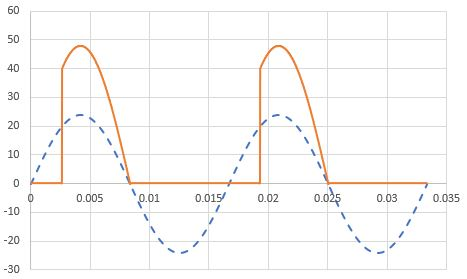
\includegraphics[width=100mm,height=\textheight]{images/ShockleyCurrentTrace.jpg}

}

\end{figure}%

\begin{itemize}
\tightlist
\item
  As the positive half-wave rises, no current flows until the incoming
  signal passes \(V_{BR_f}\).
\item
  At that point, current begins to flow, and continues to flow until the
  voltage across the device drops to practically zero.
\item
  After this, no current flows throughout the negative half cycle, nor
  throughout the beginning of the next positive cycle.
\end{itemize}

The voltage across the Shockley diode looks like the following, with the
voltage dropping to under a volt once the device is turned on.
Otherwise, the entire supply appears across it, so its voltage there
looks just like the input.

\begin{figure}[H]

\sidecaption{Shockley Output Voltage}

{\centering 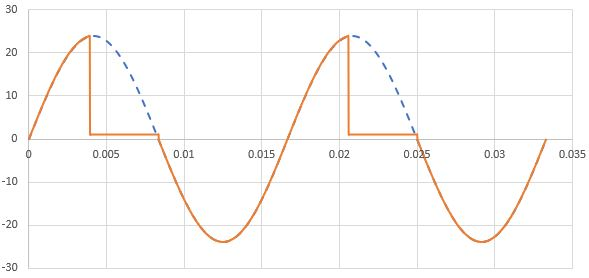
\includegraphics[width=100mm,height=\textheight]{images/ShockleyVoltageTrace.jpg}

}

\end{figure}%

As can be seen from these diagrams, power is available from somewhere
between \(90^\circ\) and \(180^\circ\) out of the total \(60^\circ\).
The greater the amplitude of the AC power or the lower the forward
breakdown for the Shockley Diode, the closer to \(180^\circ\) of
conduction, since the breakover voltage is reached earlier in the cycle.
Consequently, a Shockley Diode can only allow for less than half of the
available AC power.

\paragraph{Silicon Controlled
Rectifier---SCR}\label{silicon-controlled-rectifierscr}

\marginnote{\begin{footnotesize}

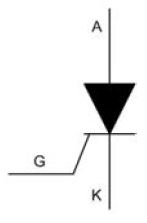
\includegraphics[width=1.04167in,height=\textheight]{images/SCRSymbol.jpg}\\
Symbol for a Silicon-Controlled\\
Rectifier (SCR)

\end{footnotesize}}

The SCR is a three-pin device that behaves like a Shockley Diode with a
controlled forward breakover voltage. The controlling pin is called a
Gate, although its function is considerably different from that of the
Gate in a FET. In the context of an SCR, the Gate ``opens'' the main
current path in response to the injection of sufficient Gate current. In
many circuits, this occurs at a voltage established using a voltage
divider that follows the voltage across the SCR. In this configuration,
once the trigger occurs and the SCR is turned On, the voltage at the
Gate drops, so no further Gate current is injected. It is no longer
needed, as the SCR remains On until the signal crosses the zero line
anyway.

With no connection to the Gate, the SCR will behave as a Shockley Diode,
but usually the forward breakover voltage is higher than the peak
voltage of the AC source. However, by injecting Gate current, the
forward breakover voltage can be lowered, turning the SCR on earlier in
the positive half-cycle.

The following transfer function shows how varying the timing of the
injection current into the Gate affects the forward breakover voltage.

\begin{figure}[H]

\sidecaption{Shockley Diode Transfer Function}

{\centering 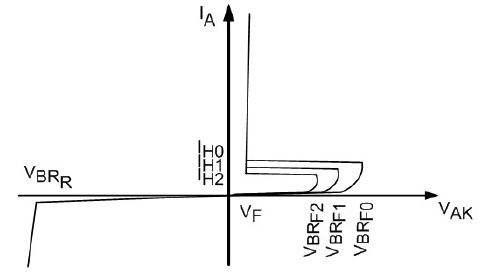
\includegraphics[width=100mm,height=\textheight]{images/SCRTransfer.JPG}

}

\end{figure}%

The graph below shows an SCR with Gate current injected to reduce the
forward breakover voltage to just under \(24 V\), then \(20 V\), and
finally to \(10 V\).

\begin{figure}[H]

\sidecaption{Shockley Output Current}

{\centering 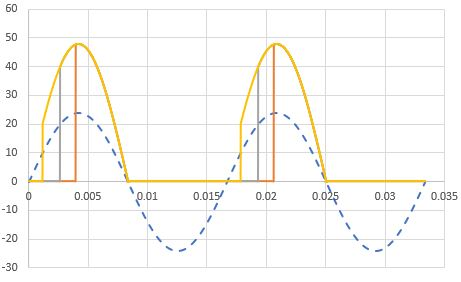
\includegraphics{images/SCRCurrentTrace.JPG}

}

\end{figure}%

Here are the voltage curves for the same settings as in the current
graphs above:

\begin{figure}[H]

\sidecaption{Shockley Output Voltage}

{\centering 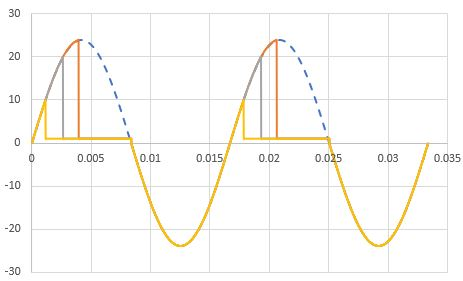
\includegraphics{images/SCRVoltageTrace.jpg}

}

\end{figure}%

As can be seen from these sets of graphs, the SCR can be adjusted to
provide between approximately \(90^\circ\) and close to \(180^\circ\)
using the Gate.

As previously mentioned, SCRs are usually chosen to have a basic
\(V_{AK}\) that is significantly higher than the peak voltage of the AC
signal so that, with no Gate current injected, the SCR will be Off. If a
voltage divider is used to control the Gate injection current, as the
voltage divider is adjusted, it will bring VAK down to where it first
starts to fire at the top of the cycle ( \(90^\circ\) ) then will move
it toward \(180^\circ\). The circuit to the right demonstrates this type
of circuit, which is a fader, but not a very good one.

\marginnote{\begin{footnotesize}

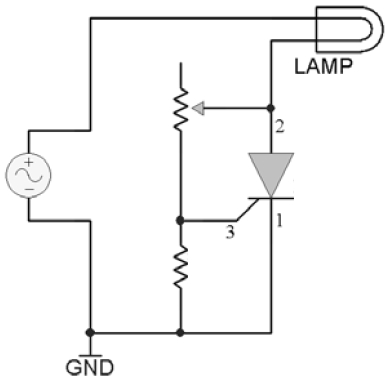
\includegraphics[width=2.08333in,height=\textheight]{images/SCRSimpleFader.jpg}\\
SCR Simple Fader Circuit

\end{footnotesize}}

The problem with this circuit is that it kicks in at \(90^\circ\) of the
available \(360^\circ\), and it can only be adjusted to increase the
conduction angle to somewhat less than \(180^\circ\). In other words, it
can adjust the power from about a quarter of the total to just under a
half -- not very impressive. We would most likely prefer to have a fader
that starts from zero and can increase the conduction angle to the
maximum available, which, for an SCR, is ideally \(180^\circ\); in other
words, from no power to half power.

Some more sophisticated fader circuits introduce circuitry to inject
Gate current at any point during the SCR's active half-cycle, allowing
for power control from zero to half of what's available from the AC
source.

\paragraph{Optoisolation}\label{optoisolation}

For both the SCR and the TRIAC (next topic), optoisolation offers at
least the following two possibilities:

\begin{itemize}
\item
  isolating high power AC circuits from low voltage DC control circuitry
  -- this will be discussed in another topic
\item
  allowing for logic-level trigger control of the AC power controller
\end{itemize}

This last item will be investigated briefly in one of our exercises. The
following is an equally brief description of the process and an
evaluation of its effectiveness in comparison to AC variable power
control.

With a comparator, it is easy to detect when the AC power signal crosses
zero volts. With an edge detector, it is possible to determine if the
crossing is from positive to negative or from negative to positive.

Since we want to be able to control the trigger time for the SCR
starting from the end of the positive half-cycle, we could create a
pulse that goes LOW at that point in time. Then, we could increase the
duty cycle of the pulse so that its positive-going edge moves forward
with respect to the negative-going crossing point, as shown in the
following graph.

\begin{figure}[H]

\sidecaption{PWM Control of an SCR}

{\centering 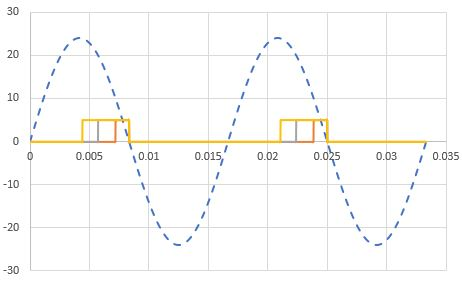
\includegraphics{images/SCRPWM.JPG}

}

\end{figure}%

This diagram shows three different pulse widths, where the red trace
would turn the SCR on for only a short time and the yellowish trace
would turn the SCR on for considerably more of the useful half-cycle,
resulting in a brighter output in a fader application. This type of
control is not possible using variable resistors and capacitors, and can
be much more carefully controlled.

\emph{Duty Cycle}---the duty cycle of a pulse is determined by

\(t_d=\frac{t_p}{T}\)

or, as a percent,

\(t_d=\frac{t_p}{T}\times100\%\)

where \(t_d\) is the duty cycle, \(t_p\) is the pulse width, and
\(T=\frac{1}{f}\) is the period of the pulse.

Pulse Width Modulation (PWM) is the process of varying the duty cycle of
a pulse, and is the term applied to the process described above.

\paragraph{Other Four-Layer Devices}\label{other-four-layer-devices}

The SCR is by far the most commonly used four-layer device. There are,
however, two other devices you may run into:

Programmable Unijunction Transistor (PUT) -- this one is really badly
named: with four layers, it has three junctions, not one; and it's only
``programmable'' in terms of the designer being able to change its
electrical conditions externally. It gets its name because it behaves
somewhat similarly to a Unijunction Transistor (UJT), which, in turn, is
similar to a JFET. All three of these share the characteristic of having
an external pin that can turn them OFF. So, unlike the SCR, once the PUT
triggers and is in its On condition, the external circuitry can turn it
off before the end of the positive half-cycle.

Silicon-Controlled Switch (SCS)---this one has two Gates---one to
control when it turns ON, like an SCR, and one to control when it turns
OFF, like a PUT.

We will not further investigate these devices in this course. They are
usually reserved for some pretty specialized control circuits.

\subsubsection{Full-Wave AC Power
Controllers}\label{full-wave-ac-power-controllers}

Modern AC Power Controllers are usually five-layer devices, which allow
control of the full (positive and negative) AC wave. Although they may
look like they could be installed either way up in a circuit, the
polarity actually matters---be sure to read the manufacturer's data
sheet! This author believed what he had been told about a two-transistor
model of the TRIAC, and ended up with pieces of hot plastic bouncing off
the walls while working on his SAIT final project because the Gate was
\(180^\circ\) out of phase from what it should have been!

\paragraph{DIAC}\label{diac}

\marginnote{\begin{footnotesize}

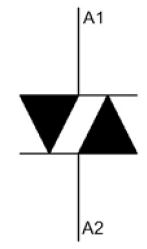
\includegraphics[width=1.04167in,height=\textheight]{images/DIACSymbol.jpg}\\
Symbol for a DIAC

\end{footnotesize}}

The DIAC is the full-wave equivalent of the Shockley Diode---it breaks
over both at a relatively high positive voltage on the positive half
wave and at a relatively high negative voltage on the negative half wave
of an AC signal.

Note that the two pins are both Anodes---\(A_1\) and \(A_2\). These
devices have nothing labelled as a Cathode.

The transfer function for a DIAC looks like the following:

\begin{figure}[H]

\sidecaption{DIAC Transfer Function}

{\centering 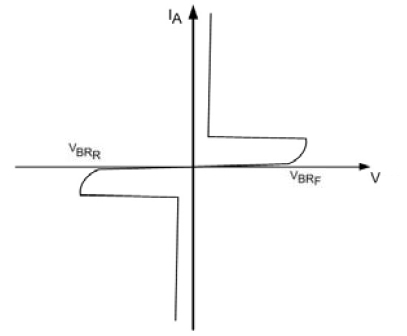
\includegraphics[width=4.16667in,height=\textheight]{images/DIACTransfer.JPG}

}

\end{figure}%

Note that \(V_{BR_r}\) for this device is not a reverse breakdown in the
sense we've used it before -- it's a reverse breakover voltage which
triggers the device into an \emph{On} condition in the negative
direction, producing a significant current over a fairly small device
voltage.

The following shows the current generated by a DIAC with forward and
reverse breakovers of \(\pm20 V\), under the same conditions as the
Shockley Diode investigated earlier.

\begin{figure}[H]

\sidecaption{DIAC Output Current}

{\centering 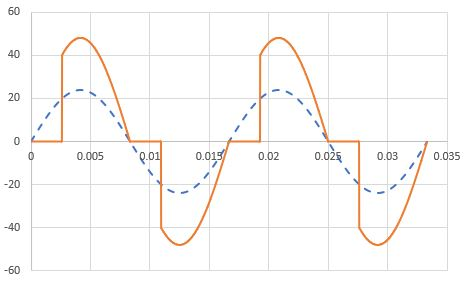
\includegraphics{images/DIACCurrentTrace.JPG}

}

\end{figure}%

The following shows the voltage curve expected for the DIAC in the
current graphs above. As with the Shockley Diode, once the DIAC has
turned on, the voltage across it drops to under \(\pm1 V\); otherwise,
the entire source voltage appears across it as it acts as an Open in the
circuit.

\begin{figure}[H]

\sidecaption{DIAC Output Voltage}

{\centering 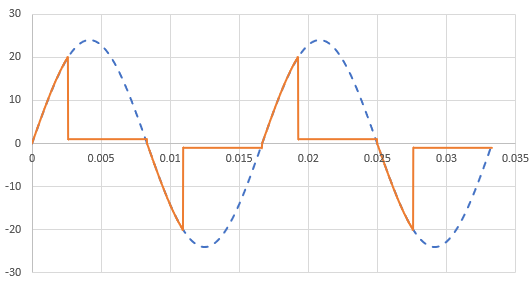
\includegraphics{images/DIACVoltageTrace.png}

}

\end{figure}%

\paragraph{TRIAC}\label{triac}

\marginnote{\begin{footnotesize}

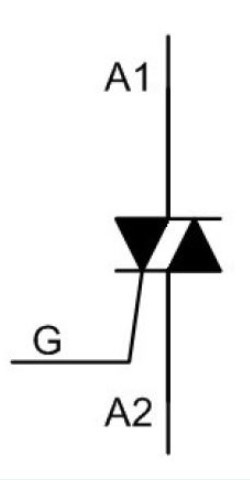
\includegraphics[width=1.04167in,height=\textheight]{images/TRIACSymbol.JPG}
Symbol for a TRIAC

\end{footnotesize}}

The TRIAC is the full-wave equivalent to the SCR -- a device with a Gate
to control both the forward and reverse breakover voltages.

Here is a typical transfer function for a TRIAC:

\begin{figure}[H]

\sidecaption{DIAC Transfer Function}

{\centering 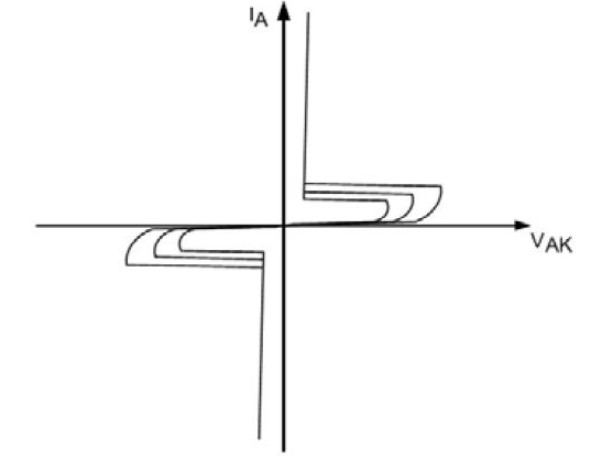
\includegraphics[width=3.125in,height=\textheight]{images/TRIACTransfer.JPG}

}

\end{figure}%

The following shows a TRIAC with basic breakover voltages much higher
than the peak voltage of the power signal, with Gate current injected to
trigger the device at just under \(24 V\), then \(20 V\) and finally
\(10 V\).

\begin{figure}[H]

\sidecaption{TRIAC Output Current}

{\centering 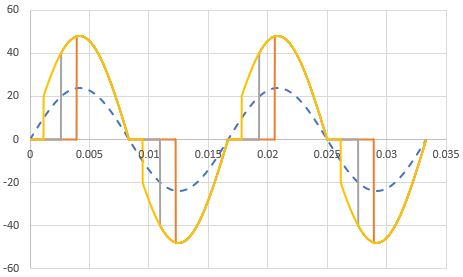
\includegraphics{images/TRIACCurrentTrace.JPG}

}

\end{figure}%

Here are the matching voltage curves for the current curves in the graph
above:

\begin{figure}[H]

\sidecaption{TRIAC Output Voltage}

{\centering 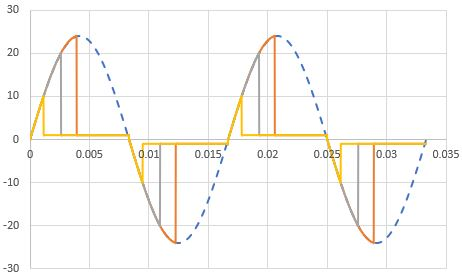
\includegraphics{images/TRIACVoltageTrace.JPG}

}

\end{figure}%

Notice that, when the TRIAC is set to turn on for most of the cycle, the
signal looks like just short spikes following the zero crossing points
of the incoming signal, then the device remains turned on until the next
zero crossing point.

When connecting a modern TRIAC in a circuit, the Gate phase needs to be
matched to the \(A_1\) anode.

\marginnote{\begin{footnotesize}

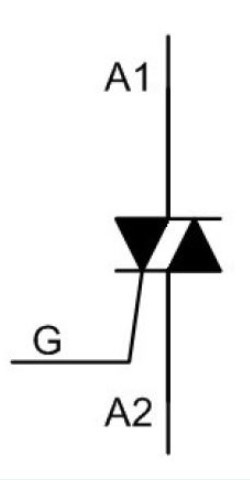
\includegraphics[width=1.04167in,height=\textheight]{images/TRIACSymbol.JPG}\\
Symbol for a TRIAC

\end{footnotesize}}

As with the SCR, the TRIAC can be used in a power fader. Assume the
TRIAC chosen has inherent breakover voltages that are greater than the
peak voltage of the power signal. With no Gate current injected, the
TRIAC will be Off. If the Gate current is injected using a controllable
voltage divider, the TRIAC can be triggered to turn on from just about
\(90^\circ\) to \(180^\circ\), then to turn on again from just about
\(270^\circ\) to \(360^\circ\). That means that, once the TRIAC is
triggered, the minimum power delivered to the load will be just over
half the total available. A fader circuit like this can provide power
control from half to full power, but not from zero to half power. With
more sophisticated circuitry, the starting angles can be moved towards
\(0^\circ\) and \(180^\circ\), allowing for a full control from
\(0^\circ\) to \(360^\circ\). The TRIAC doubles the amount of power that
can be delivered by an SCR.

In many TRIAC faders, a DIAC is used to trigger the Gate so that the
current into the Gate is turned on suddenly when the DIAC breaks over,
producing a much more reliable \emph{On} starting condition. Without the
DIAC, a TRIAC fader will typically flicker at low power settings.

\paragraph{Optoisolation}\label{optoisolation-1}

As with the SCR, optoisolators with light-activated TRIACs are
available. These can be used simply to turn a power TRIAC on or off.
However, as with the SCR optoisolator, it is possible to synchronize a
pulse width modulator (PWM) to both the positive-going and
negative-going zero crossing points of the AC power signal to provide
carefully-managed full power control. In order to establish full-wave
power control, the pulse width modulation would look something like the
following:

\href{PWM\%20Control\%20of\%20a\%20TRIAC}{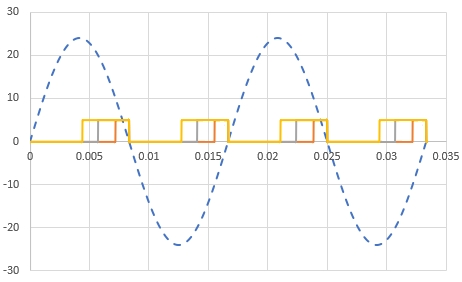
\includegraphics{images/TRIACPWM.jpg}}

\subsubsection{Optically-Isolated Power
Controllers}\label{optically-isolated-power-controllers}

In a Smart Home application or a PLC-controlled industrial process, some
form of logic circuit or microcontroller will be used to control an
AC-powered device. Although other devices such as relays and solid state
relays (SSR) could be used, often an SCR or a TRIAC is used as an
inexpensive and quiet alternative.

To protect the logic circuit or microcontroller, the circuit should be
optically isolated. Just as was the case for controlling power
transistors, optocouplers have been designed for SCR and TRIAC circuits.

In one of your projects, you will be using a TRIAC optocoupler to
activate a TRIAC in a circuit similar to the one below. Note that this
is an ON/OFF only circuit---more complex circuitry would be required to
produce a power range such as that needed for a power fader.

Since the concept is the same for an optically-isolated SCR, you haven't
been asked to purchase an SCR optocoupler. Typically, designers opt for
TRIACs in power controllers due to the extra power available anyway, so
SCR optocouplers are not as readily available as TRIAC optocouplers.

\begin{figure}[H]

\sidecaption{Optoisolated TRIAC Switching}

{\centering 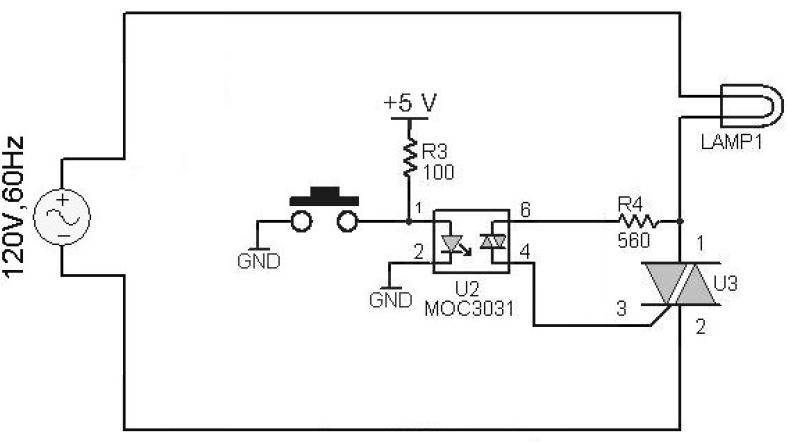
\includegraphics{images/TRIACOptocoupled.jpg}

}

\end{figure}%

In this circuit, the switch forms an \emph{Active-Low} logic switch. It
could be replaced by an NPN transistor driven by the logic circuit or
microcontroller, in which case the transistor would be capable of
providing sufficient current to turn on the LED in the optocoupler,
while the much smaller Base current required to turn on the transistor
would not load the logic circuit or microcontroller.

\begin{enumerate}
\def\labelenumi{\arabic{enumi}.}
\tightlist
\item
  When the switch in the above circuit is OPEN, current will
  \_\_\_\_\_\_\_\_\_\_ (Flow/Not Flow) through the LED, and the
  optocoupler's TRIAC will \_\_\_\_\_\_\_\_\_\_ (activate/not activate)
  the power TRIAC, and the Lamp will \_\_\_\_\_\_\_\_\_\_ (glow/not
  glow).
\item
  If the switch was to be replaced by a 2N3904 BJT, driving the
  properly-biased Base HIGH would put the transistor into
  \_\_\_\_\_\_\_\_\_\_ (cutoff/saturation) , the LED would
  \_\_\_\_\_\_\_\_\_\_ (glow/not glow) , and, following the circuit
  through, the Lamp would \_\_\_\_\_\_\_\_\_\_ (glow/not glow).
\item
  A better circuit could be built by putting the 2N3904 transistor
  between optocoupler pin 2 and ground. Now, driving the Base HIGH would
  put the transistor into \_\_\_\_\_\_\_\_\_\_ (cutoff/saturation), and
  the Lamp would \_\_\_\_\_\_\_\_\_\_ (glow/not glow) .
\item
  In the circuit of question 2, if the microcontroller was accidentally
  disconnected, the Lamp would \_\_\_\_\_\_\_\_\_\_ (glow/not glow) .
  Consequently, from a power consumption and safety perspective, the
  safer circuit is \_\_\_\_\_\_\_\_\_\_(circuit 2/circuit 3).
\end{enumerate}

\newpage{}

\subsection{Self-Test Answers}\label{self-test-answers}

\begin{enumerate}
\def\labelenumi{\arabic{enumi}.}
\item
  \begin{itemize}
  \tightlist
  \item
    flow
  \item
    activate
  \item
    glow
  \end{itemize}
\item
  \begin{itemize}
  \tightlist
  \item
    saturation
  \item
    not glow
  \item
    not glow
  \end{itemize}
\item
  \begin{itemize}
  \tightlist
  \item
    saturation
  \item
    glow
  \end{itemize}
\item
  \begin{itemize}
  \item
    glow
  \item
    circuit 3
  \end{itemize}
\end{enumerate}




\end{document}
